% !Mode:: "TeX:UTF-8" 

\BiChapter{研究可编程设备加速网络硬件交换层方法}{Switch} %15页


\BiSection{本章引论}{aa}


\BiSection{问题背景}{aa}

可编程网络硬件可以运行传统部署在服务器内的功能,从而将网络性能提高数个量级。由于软件定义网络概念的提出,网络灵活性增强,运营商更倾向于自主管理网络内设备的所有行为。具有灵活性的管理方式可以大大增加网络的运行效率,为特定的功能定制专用的网络场景。  现有的面向网络通信的可编程数据平面一般有x86平台,开放接口配置的ASIC转发芯片,以及上一章本文提到的FPGA平台。他们在处理灵活性,转发性能等方面均有长足进步,但正如本文第二章中介绍,在面对转发容量进一步增强,灵活性需求进一步开放的网络应用时依然面临新的挑战:

1)软件具有高度灵活性,但处理性能低下。

数据包交换对于CPU架构平台来说是一种很低效的机械劳动。在软件层面,数据包转发算法已经被优化的极为高效,但面对无穷无尽的任务量,依靠CPU指令集的处理架构存在访存效率低、无法批处理等问题。CPU无法发挥自己实现灵活程序跳转、分支的优势,因此目前高性能软件网络处理性能也只能达到10Gbps(单核心)。对于现代服务器面向200G接口,汇聚层交换转发动辄5、6Tbps的性能需求是远远无法满足的。

2)基于FPGA可编程硬件平台。

FPGA是一种逻辑可编程芯片,可提供软件一般的灵活性也具有硬件的性能。目前,主要的云计算厂商阿里巴巴、亚马逊、微软都在数据通路内部署了FPGA加速引擎以同时满足性能和灵活性的需求,例如提升网络加解密性能,定制传输层协议等。然而由于FPGA电路编码转换采用“查找表+内部互联网络”的原理,为保证时间同步性,使得FPGA综合对外的处理主频只能达到200MHz,这样即使FPGA内流水线每个周期都能处理一个数据包,总吞吐性能也无法超过100Gbps\citeup{wang2017p4fpga,netfpga2014}。虽强于软件,但远差于网络的核心层性能需求。

3)协议无关概念的交换芯片。

与协议无关交换架构(Protocol-Independent Switch Architecture,PISA)相对应的是P4(Programming Protocol-Independent Packet Processor)。P4是一种专用的编程语言,其目标是为任意包协议提供一种基于ASIC硬件(PISA)的现场可重配置能力。根据本文在第二章的介绍,PISA有能力实现自定义包头解析,自定义流表的组成结构,并且最重要的它拥有最强大的处理能力(12.8Tbps,显然是唯一可以胜任核心转发设备的架构)。虽然这大大解决OpenFlow编程能力不足以及其设计本身所带来的的可扩展性差的难题,但它不具备真正意义上其所追求的“图灵完备”可编程。例如:(1)数据通路内的处理动作只能被数据包触发,而无法响应其他行为。针对一些QoS场景系统更希望根据队列深度做出一些响应,比如拥塞控制场景下的控制算法NDP\citeup{handley2017re};(2)PISA缺乏计算、控制属性的指令集,例如乘除法、灵活分支判断等;(3)PISA为无状态转发的可编程流水线设计,则对状态协议处理以及有状态计算造成了困难(防火墙等)。

PISA转为通用型的无状态转发同时提高了性能与灵活性,本文将对PISA架构芯片的目标处理内容做进一步扩展。本文的目标是设计一种适用于网络交换层的交换机架构,这种架构可从计算平面高灵活性的工作任务分离和卸载到网络中,包含但不限于有状态转发、复杂计算以及自定义触发方式。



\BiSection{系统架构介绍}{aa} 

P4是目前广泛使用的可定义数据平面内的数据包解析和查表过程的语言。P4将流水线外的功能需求通过P4\_extern模块来让用户自行定义。然而P4\_extern的编程范围只在PISA提供的执行器序列之内,例如校验算法,位移,插入数据等。目前的PISA芯片架构对于“PISA\_extern”的功能需求没有支撑能力。一种显而易见的解决方案是当需要一种新的“PISA\_extern”时,重新设计一种支撑新特性执行器的ASIC硬件。但这与PISA高灵活性的设计初衷相矛盾,从经济实用性角度分析也是不合理的。

本文提出一种硬件异构型的交换机架构,可以支持任意P4\_extern所定义的功能。本文将这种结构命名为“自适应交换”,首先本文需要解决如何设计硬件结构使得灵活性和性能可以充分展现,其次本文需要解决如何开发编程语言以映射到自适应交换的数据平面。最终为了展示自适应交换的高扩展性,本文将上小节内提出的PISA难以应用的场景均在自适应交换平台中实现。

\BiSubsection{架构设计}{aa}

\begin{figure}[!ht]
	\centering 
	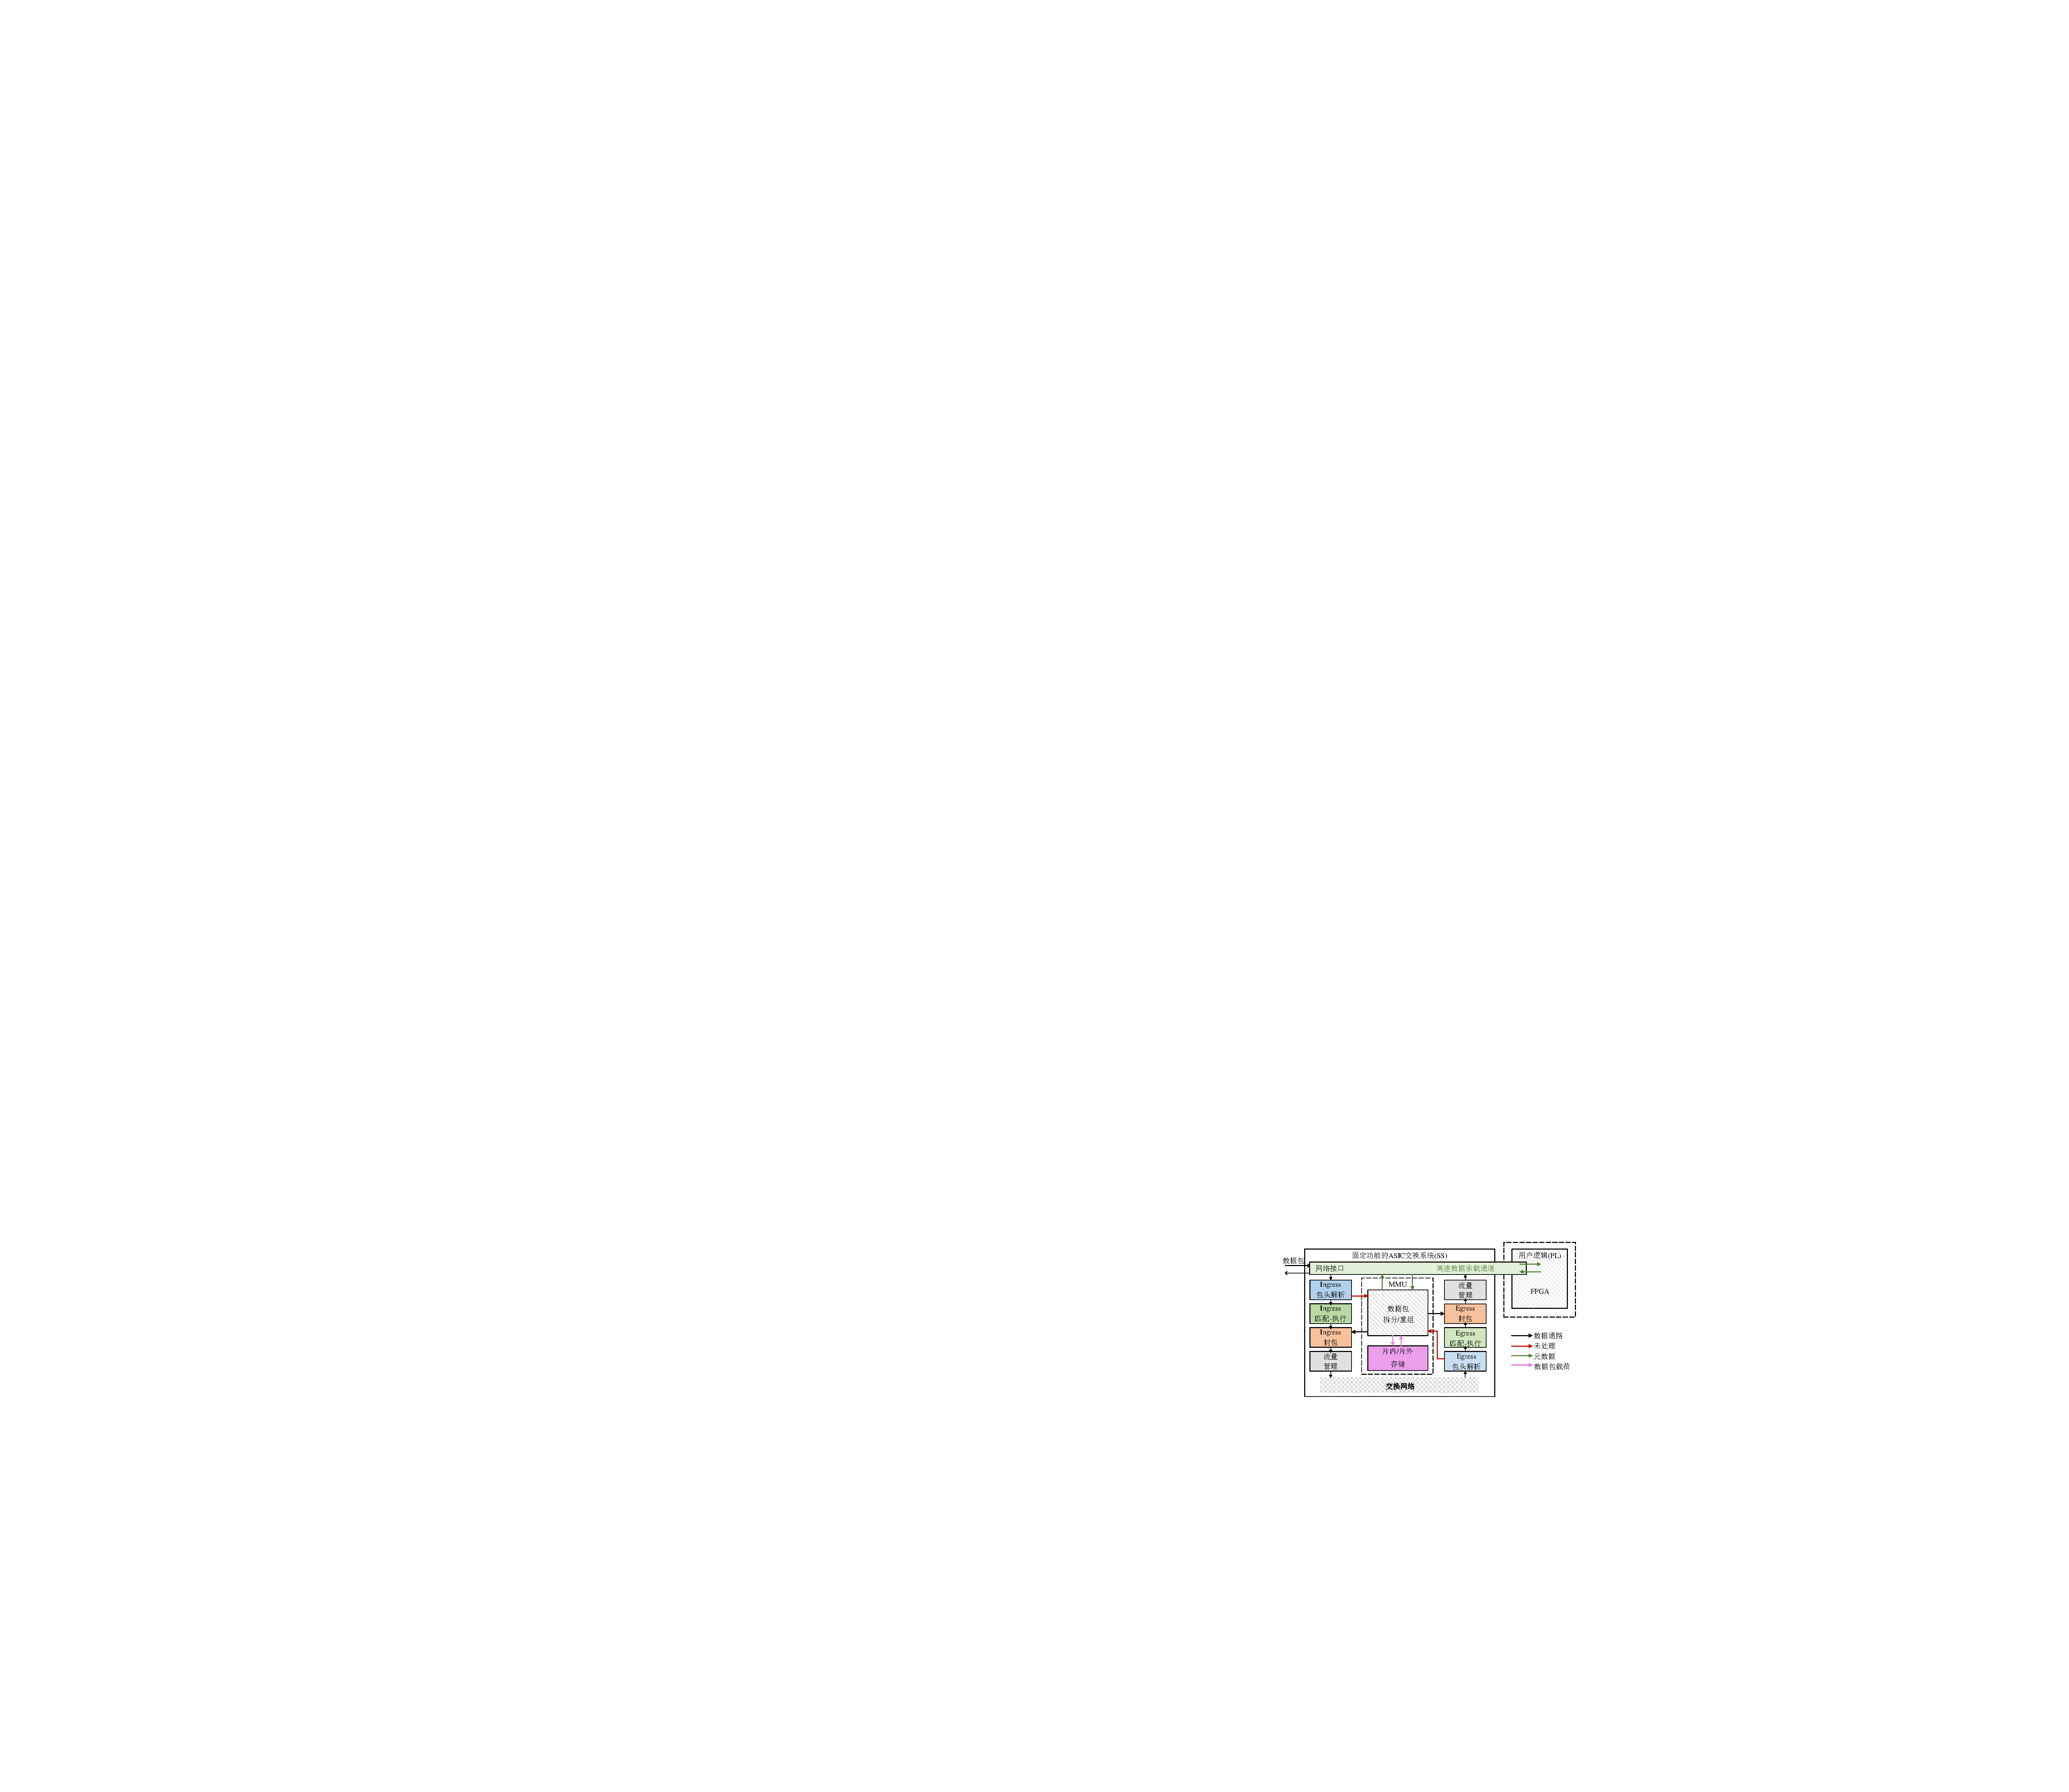
\includegraphics[scale=1]{asarch.pdf}
	\caption{自适应交换结构框图} \label{fig:asarch}
\end{figure}

自适应交换的硬件架构框图。自适应交换包括两部分,1)固定功能的ASIC交换系统(Switching System, SS);2)用户定义可编程逻辑块(Programmable Logic, PL)。SS基于标准的交换芯片(switching ASCI)处理功能,PL利用FPGA类的可编程硬件支持用户自定义逻辑。一个标准的交换芯片功能包含了数据包头的解析,基本的ACL功能和各个字段的匹配以及执行转发/丢包等动作。额外还会包括流量管理、队列调度等QoS功能。架构中SS与PL两部分可由双芯片拼接的方式实现,SS部分利用一个标准传统的交换芯片(既可以支持P4编程,也可以不支持P4编程)构成。PL端使用FPGA芯片或由FPGA构成的多用途片上系统(MPSoC/ACAP)芯片。在双芯片拼接方案中,两个独立的芯片系统须通过高速互联总线相连接,例如PCIe接口,以太网接口或者类似的收发器。相应地自适应交换系统也可以由单独一颗芯片构建而成,PL与SS部分通过片上高速总线相接,例如,AXI协议总线。

如图\ref{fig:asarch}左半部分所示,交换网络是SS的核心组成部分。交换网络支持网络入端接口与出端接口多对多的数据包互联传送,一般由交叉开关(cross-bar)构成。数据包经由物理网络接口进入SS系统,在交换网络两边,数据包会经过入端(Ingress)处理流水线,以及出端(Egress)处理流水线。在两条流水线的组成分别有包头解析(抽取必要的包头域数据),流表(对包头域数据进行匹配和执行相应的动作集),封包(重组/修改数据包结构),以及流量管理(包缓存/调度/限速等)。

数据包进入自适应系统时,首先经由SS端的处理,通常情况下大部分数据包可以完整地被SS处理,并返回外部网络。只有在SS内的功能无法满足需求的那部分数据包会再次送入PL端做协同处理。对于送往PL端处理的数据包,在SS端在片上存储中(或使用片外存储)也保留有一份完整是数据包备份,SS只将数据包的元祖数据信息送给PL。元祖数据中包括了PL完成处理所需要的定制化的包头信息或者其他描述信息。PL处理完成元祖数据后,会更新重写元祖信息中的包头以及描述字段,再返回给SS。最后SS将备份的原始数据包与更新的元祖数据重新整合成一个完整的数据包后再次对其执行转发操作,或简单丢包。

本文将在传统的交换芯片中增加一个包存储管理机制(Memory Management Unit, MMU),图\ref{fig:asarch}中左边虚线内部所示。当数据包元祖信息送往PL处理时,这个数据包在SS端的完整备份由MMU管理。MMU应包含三个主要功能:(1)动态申请/释放数据包的存储块位置及其大小;(2)驱动数据包向内存中读写时序;(3)读出备份数据包后与从PL返回的新元数据对接重组。

上述自适应交换流程与原理是建立在本文对以下两方面的分析结果和假设之上。首先,在PL中处理的信息通常只依赖于包头,或者数据包包首部分的字段。在设计中被交换到PL的元数据可以被灵活地定义,并且保证只占用SS与PL之间一定量的通信带宽成本。在某些极端的例子中,如果处理过程需要数据包所有的数据时,元祖数据也将会包含一个完整的数据包内容。第二,不是所有的数据包处理都需求调用PL端的功能。否则,如果有一种功能是普遍适用的,则一定会集成在现行的通用交换芯片内。或者这种功能需求可以直接拆分出来一部分由SS端完成处理。

自适应交换的高性能来自于对网络通用数据包包长的分析。本文考虑到,目前网络内平均包长度为600字节左右,假设元祖数据包含整个包头部分(64字节之内),则SS与PL之间的通信成本只占需求流量的10\%。即,利用单插槽的PCIe4.0接口(256Gbps)作为高速互联,自适应交换系统可以将目前最高速度(12.8Tbps)交换芯片中20\%的数据(>2Tbps)卸载到用户硬件可编程逻辑中进行处理。这远远超过了($\times$10倍)单纯由FPGA组成的可编程数据平面的处理性能,也是本文研究的最主要的动机。

\BiSubsection{开发流程}{aa}

对于基于FPGA的PL端,基本的开发设计流程包括如下几部分:

\begin{itemize}
	\item 定义数据包处理需求以及所需要的数据流模型。
	\item 编写处理规则对应的函数或流程代码。程序代码可包括高级语言如P4/P4\_extern、P4\_FPGA,或者底层的硬件描述语言如verilog HDL。此外包括数据平面高层次生成系统,如SDNet\citeup{sdnet},也可以用于加速PL端的开发工作。
	\item PL端的机器码编译器。不同PL目标器件下的编程,往往有不同的编译步骤。对于基于FPGA的编译器,本文使用FPGA芯片厂商提供的编译环境。但本文最主要的贡献是解决如何将数据包流处理模型在异构形态下重新组织,并且完成高性能的异构形态下包处理逻辑无语义偏差的拆分和翻译。
\end{itemize}

\begin{figure}[!ht]
	\centering 
	
\includegraphics[scale=1]{asdev.pdf}
	\caption{基于FPGA的PL开发流程} \label{fig:asdev}
\end{figure}

本文利用Xilinx SDNet/P4-SDNet作为建立本文设计原型系统的基本开发工具,基于FPGA的PL编译流程如图\ref{fig:asdev}所示。SDNe



\BiSection{硬件设计}{aa}

各种花哨 映射方法,加速方法

rmt的crossbar介绍

有状态转发

\BiSection{软件设计}{aa}

NP难题


\BiSection{系统性能评价}{aa}





\BiSection{本章小结}{aa}





